%%letter, article, report, book
\documentclass[12pt]{article}

\usepackage{listings}
\usepackage{comment}
\usepackage{graphicx}
\usepackage{subfigure}

\usepackage[margin=1in]{geometry}
\usepackage{setspace}
\usepackage{harvard}

\begin{document}
	\title {Radiomic feature extraction}
	\author {Valeria Amato}
	\date{20/12/2021}

	\maketitle

	\begin{abstract}
This report describes a framework able to extract radiomic features, thanks to the open-source python package: pyradiomics (1).
Radiomic data has the potential to uncover disease characteristics that fail to be appreciated by the naked eye.
The central hypothesis of radiomics is that distinctive imaging algorithms quantify the state of diseases, and thereby provide valuable information for personalized medicine. 
The paper defines how to extract lung tumor nodules characteristics, which are in The Cancer Imaging Archive, exactly in the collection LIDC-IDRI.
The framework provides a simple interface for the extraction of the main features by only inserting paths to the DICOM directories.
	\end{abstract}

	\section{Introduction}\label{sec:intro}
The framework is able to extract radiomic features, thanks to the open-source python package: pyradiomics (1). 
This package establishes a reference standard for Radiomic Analysis, and provide a tested and maintained open-source platform for easy and reproducible Radiomic Feature extraction(Warning: not intended for clinical use.).The platform supports both the feature extraction in 2D and 3D and can be used to calculate single values per feature for a region of interest.

The framework is implemented to extract features from the LIDC-IDRI dataset in The Cancer Imaging Archive (TCIA), a service which de-identifies and hosts a large publicly available archive of medical images of cancer.  TCIA is funded by the Cancer Imaging Program (CIP), a part of the United States  National Cancer Institute (NCI), and is managed by the Frederick National Laboratory for Cancer Research (FNLCR).
line

	\pagebreak
	\section{How to use it?}\label{sec:use}
	\subsection{Setup}\label{sub:install}
	\subsubsection{Cancer Imaging Archive - Data Download}
The imaging data in The Cancer Imaging Archive are organized as “collections” defined by a common disease (e.g. lung cancer), image modality or type (MRI, CT, digital histopathology, etc) or research focus. 
DICOM is the file format used by TCIA for LIDC-IDRI.

Once in the LIDC-IDRI dataset in The Cancer Imaging Archive, add in the chart a collection ID and download it. 

If it is the first time, you may not have installed the NBIA Data Retriever on your computer.
You must install the NBIA Data Retriever before you begin downloading. You only have to install it once to use it in future downloading sessions.

From this point, you must have installed NBIA Data Retriever.

When the download of the TCIA file is completed, click on it and let NBIA open it.
You must agree to the data usage policy before you can proceed with downloading the data in your cart. Note that this policy is included in the license file accompanying your download.

Select directory type for downloaded files: Classic Directory Name
Select directory for downloaded files.
Start.

\begin{figure}[h]
	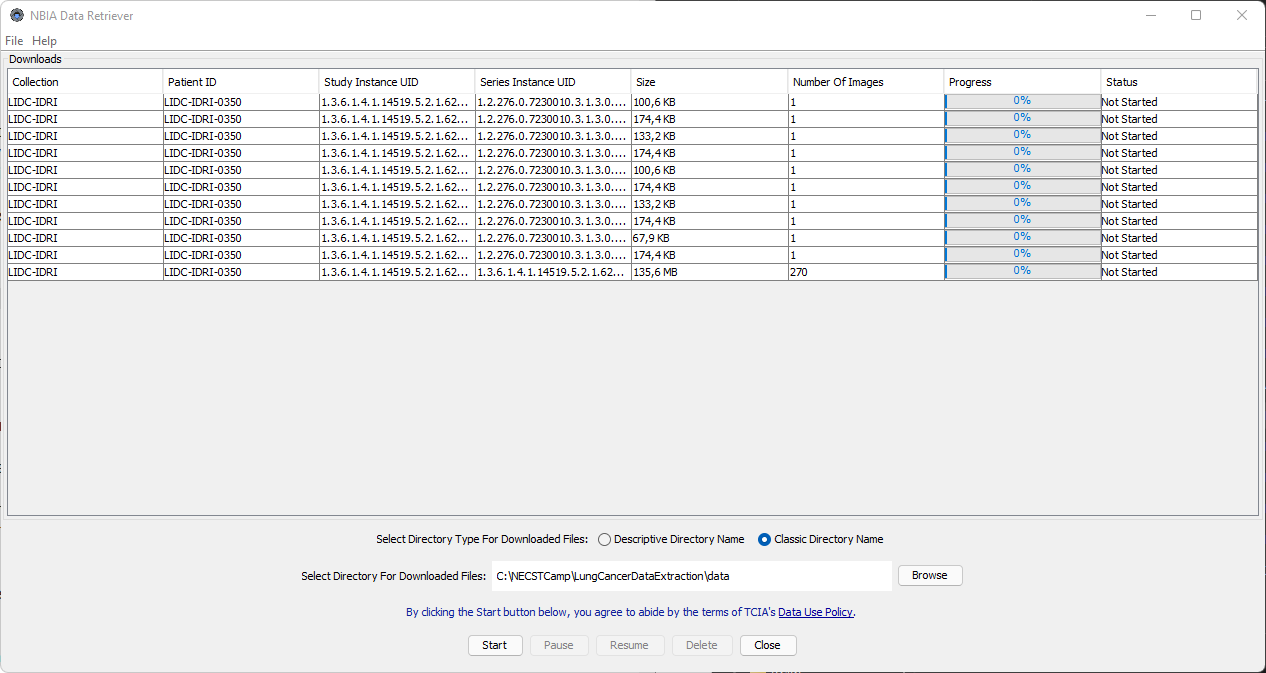
\includegraphics[ width=17cm]{NBIA}
	\caption{A screenshot of NBIA Data Retriever with a TCIA file to load. 
	Note: Classic Directory Name preferred }
\end{figure}

Now, you can access to the dicoms directory.
\begin{comment}
	\subsubsection{Data organisation}
The framework uses many pylidc \cite{pylidc} functions that do require access to the DICOM files associated with the LIDC dataset. 

Pylidc requires a special configuration file that tells it where DICOM data is located on your system.

pylidc looks in your home folder for a configuration file called, .pylidcrc on Mac and Linux, or pylidc.conf on Windows. You must create this file. On Linux and Mac, the file should be located at /home/[user]/.pylidcrc. On Windows, the file should be located at C:Users[User]pylidc.conf.

The configuration file should be formatted as follows:
\begin{listing}
[dicom]
path = /path/to/big_external_drive/datasets/LIDC-IDRI
warn = True
\end{listing}

\end{comment}
\linebreak
The setup is finished.
	\pagebreak
	
	\section{Script clarification}\label{sec:clary}
	\subsection{Inputs}
	
The inputs required are used to locate dicoms and metadata inside the directory. 
Pay attention do not cause the unicode error, for example not using two backslashes (\\) for the path.

	\subsubsection{dirName}
The variable dirName indicates the path to the DICOMs folder. 
In some cases, there are collection with more studies and multiple series inside each study. 
However, only one serie is complete of xml and many DICOMs. 
Take that path.

	\subsubsection{pid}
The variable pid is a string which has the corresponding patientID.

	\subsubsection{imagePath}
The string imagePath indicates the path in which converted DICOMs will be stored.
The conversion is from a series of DICOMs into a SimpleITK object (NRRD) that can be read by the pyradiomics (1) package.

	\subsubsection{maskPath}
The string maskPath indicates the path in which the 3D mask (file format: NRRD) of the volume is stored.

	\subsection{Extraction}
Once all DICOMs have been loaded and converted into NRRD, the script extract the mask from the XML file referring to the patientID.

\begin{figure}[htp]

\centering
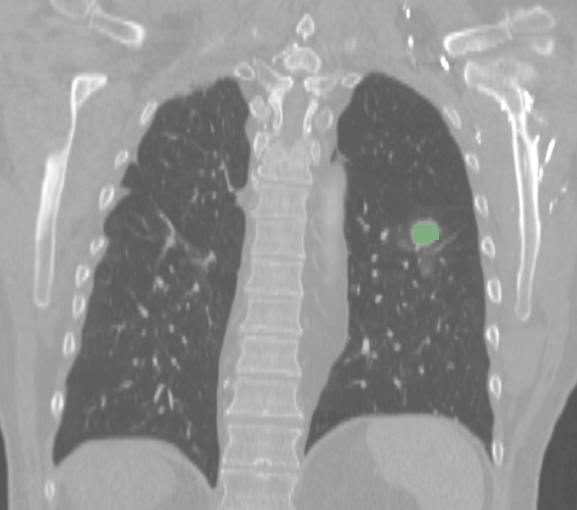
\includegraphics[width=.3\textwidth, height = 4cm]{LUNG1}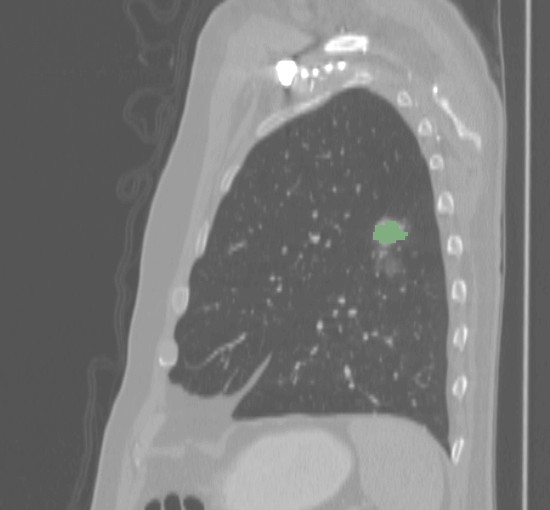
\includegraphics[width=.3\textwidth,  height = 4cm]{LUNG2}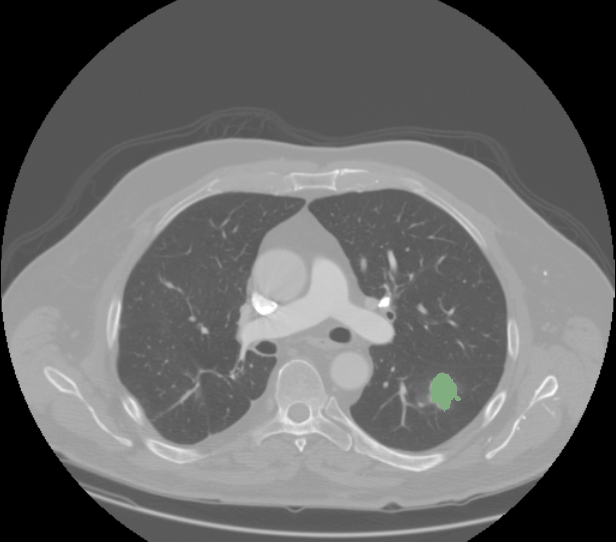
\includegraphics[width=.3\textwidth,  height = 4cm]{LUNG3}

\caption{Three sides of lung image with the segmented mask (green).}

\end{figure}
Then, the extraction can begin.

The extraction has the following parameters:
	\begin{itemize}
		\item minimumROIDimensions: 2
		\item minimumROISize: None
		\item normalize: False
		\item normalizeScale: 1
		\item removeOutliers: None
		\item resampledPixelSpacing: None
		\item interpolator: 'sitkBSpline'
		\item preCrop: False
		\item padDistance: 5
		\item distances: [1]
		\item force2D: False
		\item force2Ddimension: 0
		\item resegmentRange: None
		\item label: 1
		\item additionalInfo: True
	\end{itemize}
and any filter is applied.

	\subsection{Outputs and Results}
	\subsubsection{No DICOMs in the directory}
The script prints on stdout the absence of DICOMs and ends.

	\subsubsection{Features extracted}
All features enabled (extracted):
	\begin{itemize}
		\item firstorder
		\item glcm
		\item gldm
		\item glrlm
		\item glszm
		\item ngtdm
		\item shape
	\end{itemize}

	\pagebreak
	\section{Conclusion}\label{sec:con}
The framework is able to extract various statistics, which are singly explained below.

	\subsection{First Order Feature}
First-order statistics describe the distribution of voxel intensities within the image region defined by the mask through commonly used and basic metrics.

	\subsection{Gray Level Co-occurrence Matrix (GLCM) Features}
A Gray Level Co-occurrence Matrix (GLCM) of size N×N describes the second-order joint probability function of an image region constrained by the mask.

	\subsection{Gray Level Dependence Matrix (GLDM) Features}
A Gray Level Dependence Matrix (GLDM) quantifies gray level dependencies in an image. A gray level dependency is defined as a the number of connected voxels within distance that are dependent on the center voxel. 

	\subsection{Gray Level Run Length Matrix (GLRLM) Features}
A Gray Level Run Length Matrix (GLRLM) quantifies gray level runs, which are defined as the length in number of pixels, of consecutive pixels that have the same gray level value.

	\subsection{Gray Level Size Zone Matrix (GLSZM) Features}
A Gray Level Size Zone (GLSZM) quantifies gray level zones in an image. A gray level zone is defined as a the number of connected voxels that share the same gray level intensity. A voxel is considered connected if the distance is 1 according to the infinity norm (26-connected region in a 3D, 8-connected region in 2D). In a gray level size zone matrix P(i,j) the (i,j)th element equals the number of zones with gray level i and size j appear in image. Contrary to GLCM and GLRLM, the GLSZM is rotation independent, with only one matrix calculated for all directions in the ROI.

	\subsection{Neighbouring Gray Tone Difference Matrix (NGTDM) Features}
A Neighbouring Gray Tone Difference Matrix quantifies the difference between a gray value and the average gray value of its neighbours within distance. The sum of absolute differences for gray level i is stored in the matrix. 

	\subsection{Shape}
In this group of features we included descriptors of the two and three-dimensional size and shape of the ROI. These features are independent from the gray level intensity distribution in the ROI and are therefore only calculated on the non-derived image and mask.

Unless otherwise specified, features are derived from the approximated shape defined by the triangle mesh. To build this mesh, vertices (points) are first defined as points halfway on an edge between a voxel included in the ROI and one outside the ROI. By connecting these vertices a mesh of connected triangles is obtained, with each triangle defined by 3 adjacent vertices, which shares each side with exactly one other triangle.
\begin{comment}
This mesh is generated using a marching cubes algorithm. In this algorithm, a 2x2 cube is moved through the mask space. For each position, the corners of the cube are then marked ‘segmented’ (1) or ‘not segmented’ (0). Treating the corners as specific bits in a binary number, a unique cube-index is obtained (0-255). This index is then used to determine which triangles are present in the cube, which are defined in a lookup table.

These triangles are defined in such a way, that the normal (obtained from the cross product of vectors describing 2 out of 3 edges) are always oriented in the same direction. For PyRadiomics, the calculated normals are always pointing outward. This is necessary to obtain the correct signed volume used in calculation of MeshVolume.
\end{comment}

	\begin{thebibliography}{99}

	\bibitem{pyradiomics}
van Griethuysen, J. J. M., Fedorov, A., Parmar, C., Hosny, A., Aucoin, N., Narayan, V., Beets-Tan, R. G. H., Fillon-Robin, J. C., Pieper, S., Aerts, H. J. W. L. (2017). Computational Radiomics System to Decode the Radiographic Phenotype. Cancer Research, 77(21), e104–e107. `https://doi.org/10.1158/0008-5472.CAN-17-0339 <https://doi.org/10.1158/0008-5472.CAN-17-0339>`

	\end{thebibliography}

\end{document}